\documentclass{beamer}
\usetheme{metropolis} 
\usecolortheme{rose}

\usepackage{xcolor}
\usepackage[utf8]{inputenc}
\usepackage{hyphenat}
\usepackage[russian,english]{babel}          % Use metropolis theme

\setbeamertemplate{footline}[frame number] % указывает на каждой странице общее количество страниц




% Указывайте все новые термины в \termdef команде. А уже известные ранее или из других курсов в \term
\newcommand{\termdef}[1]{\textbf{\textit{#1}}}
\newcommand{\term}{\textit}
% Диалог с аудиторией.
\newcommand{\auditorium}[1]{\color{red}{\textbf{#1}}}
% \setbeamercolor{auditorium}{fg=red}

\title{Лекция 2. Экспертные системы. Основные параметры качества.}
% \date{\today}
\date{9 сентября 2019}
\author{Павел Владимирович Слипенчук}
\institute{Москва, МГТУ им.Бауманка,\\ каф.ИУ-8, КИБ}
% \titlegraphic{\includegraphics[width=2cm]{logo_ur.jpg}}
\titlegraphic{\small \href{https://github.com/kib-courses/dsis}{Data Science для решения задач информационной безопасности}}

\begin{document}
  \maketitle
    
  \begin{frame}{План лекции}
    \begin{enumerate}
	\item \nameref{section:classification_defs}
	\item второе
	\end{enumerate}
 \end{frame}
    
  \section{Признак. Вектор признаков Классы. Обучающая и тестовая выборки. Задача классификации, классификатор(оценщик)}\label{section:classification_defs}
  
  \begin{frame}{Признак, вектор, класс}
    \termdef{Признак} $x_i$-- определенное значение. Категориальное, сравнимое, или числовое: целочисленное, булевое, или дробное.
    
    \termdef{Вектор признаков} $\bold x = (x_1, x_2, ... x_n)$ -- вектор, каждое значение которого является \term{признаком}. 
  	
  	\termdef{Класс} (метка) $y$ -- значение (как правило целочисленное), присваиваемое какому-либо вектору признаков: $ y \mapsto \bold x$
  	
  	\auditorium{А в чем физический смысл?}
  \end{frame}
  
  \begin{frame}{Пример}
  \begin{itemize}
  	 \item $x_1$ -- сумма транзакции [в рублях]
  	 \item $x_2$ -- возраст клиента [в годах]
  	 \item $x_3$ -- пол клиента [булевый: 1 -- мужской, 0 -- женский]
  	 \item $x_4$ -- MCC код\footnote{\termdef{Merchant Category Code} -- номер деятельности компании при осуществлении безналичной оплаты. Например \textbf{1731} означает оплату за электроэнергию, \textbf{3137} -- покупка авиабилетов, \textbf{4121} -- такси}
  	 \item  $y=1$ -- операция мошенническая (фродовая);  $y=0$ -- легитимная.
  \end{itemize}
  \begin{center}\small \begin{tabular}{ l l }\label{tabular:class_feature_vector_example}
  	$0 \mapsto (3234, 25, 1, 1731) $ &  $0 \mapsto (2540, 55, 0, 1731)$ \\
  	$1 \mapsto (18400, 45, 0, 3137)$ & $0 \mapsto (2540, 55, 0, 1731)$  \\
  	$1 \mapsto (903, 19, 0, 4121)$  & $0 \mapsto (1875, 45, 0, 4121)$  \\
  	$0 \mapsto (854, 21, 1, 4121)$  & $1 \mapsto (702, 21, 0, 4121)$  \\
  	$1 \mapsto (903, 19, 0, 4121)$  & $0 \mapsto (1875, 45, 0, 4121)$  \\
  	$0 \mapsto (28400, 41, 1, 3137)$ & $0 \mapsto (25040, 55, 0, 1731)$  \\
  \end{tabular}\end{center}
  \end{frame}
  
  \begin{frame}
   \begin{block}{Замечание}
	  В отличие от таблицы, представленной на слайде №\ref{tabular:class_feature_vector_example},
	  в данных на реальных задачах \term{вектор признаков} может состоять из $~200$ и более признаков:
	  $\bold x = (x_1, x_2, ..., x_{200}, ...)$
  \end{block}
  \end{frame}
  
  \begin{frame}{Функция высшего порядка}
  \termdef{Функция высшего порядка} -- это функция, принимающая в качестве аргументов хотя бы одну другую функцию и/или возвращающая в качестве выхода функцию.
  
  См.так же:
  \begin{enumerate}
  	\item \termdef{функциональное программирование}
  	\item \termdef{декоратор}, \termdef{фабрика декораторов}
  \end{enumerate}
  
  \end{frame}
  
  \begin{frame}{Классификация. Постановка задачи}\label{frame:classification_def}
  	Определим \term{неупорядоченную совокупность}:
  	\begin{equation}\label{eq:def_fit_sample}
  	U_{fit} = \left\{ y \mapsto \bold x  \right\}
  	\end{equation}
  	Множество \eqref{eq:def_fit_sample} будем называть \termdef{обучающей выборкой}.
  	
  	Функцию, отображающую вектор $\bold x$ в значения на интервале $[0, 1]$ будем 
  	называть \termdef{функцией скоринга}:
  	\begin{equation}\label{eq:score_def}
  	\hat{y} := score( \bold x); \hat{y} \in [0, 1]
  	\end{equation}
  	Значение $\hat{y}$ называют \termdef{откликом} \term{вектора признаков} $\bold x$.
  	
  	\termdef{Обучением} (в задаче классификации) будем называть процесс получения 
  	\term{функции скоринга}\eqref{eq:score_def} 
  	из 
  	\term{обучающей выборки}\eqref{eq:def_fit_sample}.
  	Таким образом можно определить \term{функцию высшего порядка}:
  	\begin{equation}\label{eq:fit_def}
  	score := fit (U_{fit}) 
  	\end{equation}
  \end{frame}

 \begin{frame}
	 \begin{block}{Замечание}
	 	$U_{fit}$ в общем случае это именно неупорядоченная совокупность, а не множество. Во множестве ни один элемент не может быть представлен более одного раза, а в неупорядоченной совокумности -- может. Для простоты в дальнейшем 	$U_{fit}$ будем называть множеством.
	 \end{block}
	\begin{block}{Замечание}
		Иногда функция $fit$ представляет собой \term{ленивое вычисление}\footnote{
		\termdef{Ленивые вычисления} (lazy evaluation, отложенные вычисления) -- 
		метод программной разработки функций, в которой вычисления откладывают до тех пор,
		пока не понадобится их результат.
		} и выдаёт $score$ почти мгновенно. И уже для каждого конкретного $\bold x$ функция
		$score(\bold x)$ рассчитывает \term{отклик} $\hat{y}$ на основании 
		\term{обучающей выборке} \term{} $U_{fit}$
	\end{block}
   \end{frame}
  
  
  \begin{frame}{Классификация}
  	Функция $fit$ (cм. \eqref{eq:fit_def} на слайде №\ref{frame:classification_def}) -- размечает каждую точку пространства признаков на величину от 0 до 1. Чем ближе эта величина к 1, тем <<более вероятно>> что это класс 1, чем ближе к 0 -- тем более вероятно что класс 0.
    \begin{center}
    	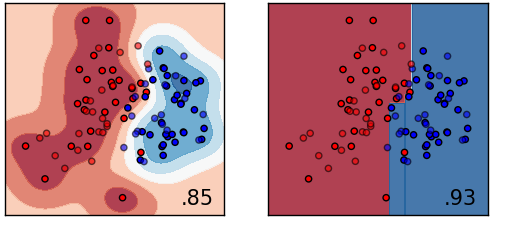
\includegraphics[width=8cm]{pic/classification_example.png}\centering
    \end{center}
	
  \end{frame}

   
   \section{Вопросы для самопроверки}

   \begin{frame}{Признаки, вектор признаков, выборка}
   \begin{enumerate}
   	\item Что такое \term{признак}?
   	\item Что такое несравнимый (категориальный) признак? Чем он отличается от сравнимого?
   	\item Что такое булевый признак? Числовой?
   	\item Приведите пример булевого и несравнимого признака. Болевого и сравнимого. 
   	\item Что такое \term{вектор признаков}? Есть два вектора $\bold x_a = (x_1, x_2)$ и $\bold x_b = (x_2, x_1)$.
   	Являются ли они идентичными? Можете привести задачу, когда являются?
   	\item Что такое \term{обучающая выборка}? Почему формула \eqref{eq:def_fit_sample} задаётся
   	как \textbf{неупорядоченная} совокупность, а не как список (т.е. упорядоченная совокупность).
   	Почему порядок перечесления данных в аргументе функции \eqref{eq:fit_def} не важен?
   \end{enumerate}
	\end{frame}

   \begin{frame}{Обучающая выборка со слайда №\ref{tabular:class_feature_vector_example}}
 	Посмотрите на \term{выборку} со слайда №\ref{tabular:class_feature_vector_example}. 
 	\begin{enumerate}
 	\item Верно ли утверждение, что если совершается оплата электроэнергии, то данная операция всегда легитимная?
 	\item Есть ли корреляция между возрастом клиента и мошенничеством при покупке авиабилетов? 
 	\item Можно ли предположить, что таксисты чаще обманывают молодых девушек? 
 	\item Покупает ли молодёжь авиабилеты через данный банк? 
 	\item Если совершают мошенничество в сфере автоперевозок, то обманывают мужчин или женщин?
	\end{enumerate}
	\end{frame}
  

\end{document}